\chapter{Fourier Theory Made Easy (?)}
\section{Uma onda sinusoidal}

Começaremos por reproduzir uma onda sinusoidal. A sua forma mais básica, como função do tempo, é dada pela seguinte expressão:
\begin{equation}
    y(t) = A\cdot \sin \left(2\pi f t + \phi\right)
\end{equation}
% Onde:
% \begin{itemize}
%     \item $A=$ a amplitude;
%     \item $f=$ a frequência;
%     \item $2\pi f t= \omega = $ a frequência angular;
%     \item $\phi =$ a fase. 
% \end{itemize}

Para o primeiro exemplo, iremos representar em MATLAB uma onda sinusoidal com amplitude 5 e frequência de 4~Hz. Para isso, é necessário definir o eixo do tempo. Neste caso, o eixo do tempo começa em zero e acaba em 1 (segundos), com incrementos de 0.01. O código que fornece a imagem é o seguinte:

\begin{lstlisting}[style=Matlab-editor, basicstyle=\small, caption={Slide 2.}, label={lst: onda sinusoidal}]
dt = 0.01;
t = 0:dt:1;
F = 4;
A = 5;
y = A * sin(2 * pi * F * t);
plot(t,y);
xlabel('Segundos');
\end{lstlisting}

\begin{figure}[!ht]
\centering
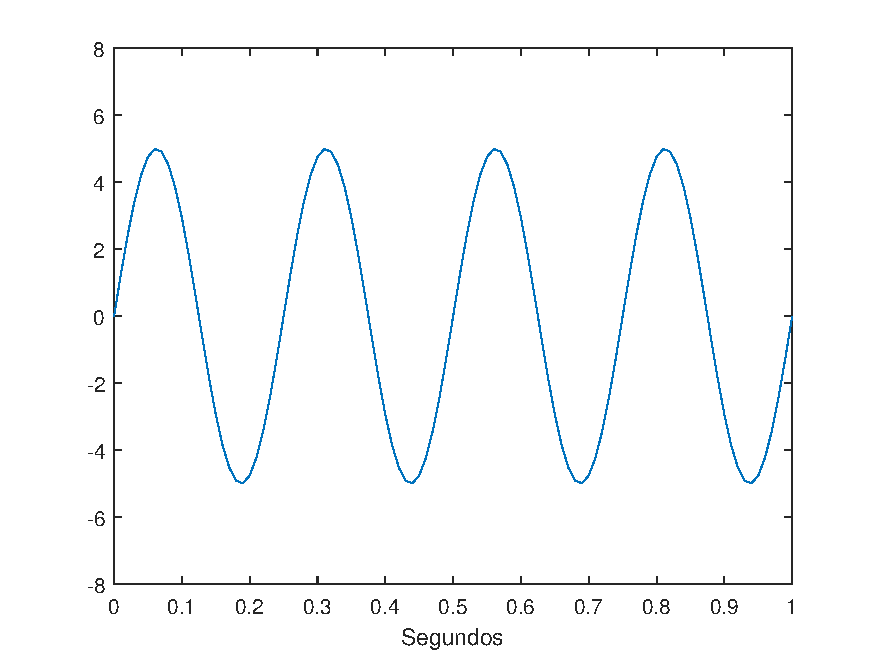
\includegraphics[width=0.75\textwidth]{onda sinusoidal.pdf}
\caption{Onda sinusoidal.}
\label{fig:onda sinusoidal}
\end{figure}

\newpage

Se definirmos a taxa de amostragem (\emph{sampling rate}) como sendo igual a 256 e a duração da amostragem (\emph{sampling duration}) como sendo igual a 1, podemos definir a variável dt como sendo o quociente entre a \emph{sampling duration} e o \emph{sampling rate}. E se representarmos a figura com pontos, podemos verificar que por cada segundo, temos 256 pontos.

\begin{lstlisting}[style=Matlab-editor, basicstyle=\small, caption={Slide 3.}, label={lst: sampling rate}]
sampling_rate = 256;
sampling_duration = 1; 
dt = sampling_duration/sampling_rate;
t = 0:dt:1;
F = 4;
A = 5;
y = A * sin(2 * pi * F * t);
plot(t, y, 'o', 'MarkerSize',4);
xlabel('Segundos')
\end{lstlisting}
    
\begin{figure}[!ht]
\centering
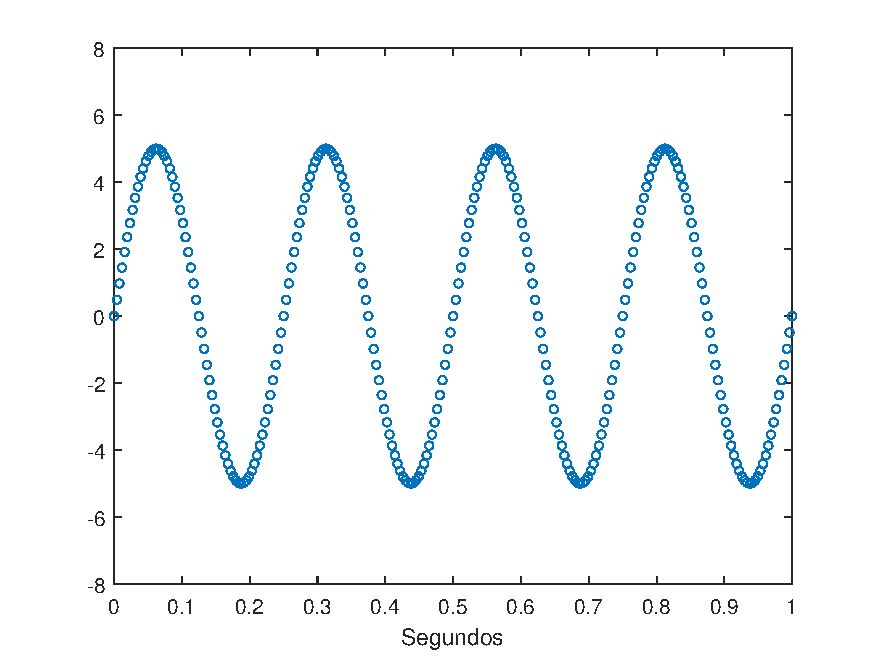
\includegraphics[width=0.75\textwidth]{samplingrate.pdf}
\caption{Taxa de amostragem.}
\label{fig:sampling rate}
\end{figure}

Agora uma função sinusoidal com frequência de 8~Hz e com uma determinada taxa de amostragem. Quando se altera o valor do passo de amostragem, para 8.5~Hz, obtêm-se um sinal com frequência de 0.5~Hz. Este exercicio, recriado em MATLAB no código da página seguinte, mostra a importância da escolha do passo de amostragem.

% Se sobrepusermos dois gráficos, um com uma taxa de amostragem muito pequena, por exemplo 8.5, e outro com uma taxa de amostragem maior, por exemplo 256, é possível verificar o efeito da taxa de amostragem. Para um eixo do tempo de dois segundos, verifica-se, na \autoref{fig:undersampled}, que no sinal subamostrado temos 18 pontos representados. 

\newpage

\lstinputlisting[style=Matlab-editor, basicstyle=\small, caption={Slide 4.}, label={lst: undersampled}, firstline=2]{./codigo/undersampled.m}

\begin{figure}[!ht]
\centering
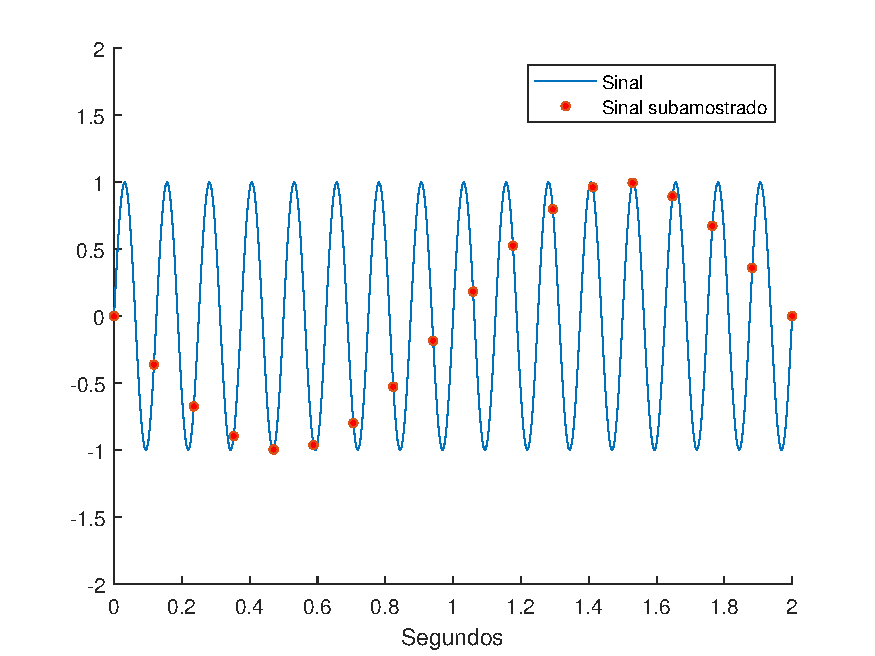
\includegraphics[width=0.75\textwidth]{undersampled.pdf}
\caption{Sinal subamostrado.}
\label{fig:undersampled}
\end{figure}

\newpage

\section{Transformadas de Fourier Famosas}

Uma transformada pega numa função (ou sinal) e transforma-a numa outra função (ou sinal).
A transformada discreta de Fourier é dada pela seguinte expressão:
\begin{equation}
    H(f)=\int_{-\infty}^{+\infty} h(t)\cdot e^{2\pi ift} \cdot dt 
\end{equation}

A transformada rápida de Fourier (do inglês: \emph{Fast Fourier Transform}, abreviado FFT), é um algoritmo que calcula a transformada discreta de Fourier. A análise de Fourier converte um sinal do domínio original (tempo) para uma representação no domínio das frequências e vice-versa.

\subsection{Função Seno \boldmath{$\rightarrow$} Função Delta} 

A transformada de Fourier de uma função sinusoidal é uma função delta de Dirac, pelo menos em parte. Quando aplicamos a transformada de Fourier no MATLAB (função \emph{fft}) a uma função sinusoidal, o resultado é uma combinação de deltas de Dirac localizados nas frequências da função sinusoidal. A transformada de Fourier da função é zero em todas as frequências exceto na frequência da função seno, onde há um Dirac localizado.

\lstinputlisting[style=Matlab-editor, basicstyle=\small, caption={Slide 12.}, label={lst: seno_delta}, firstline=2]{./codigo/seno_delta.m}

\newpage

É possível verificar pelos gráficos produzidos pelo código anterior, que o Dirac ocorre na frequência $7.98403\approx 8$, que é a frequência da função sinusoidal.

\begin{figure}[!ht]
    \centering
    \begin{minipage}[b]{0.49\textwidth}
        \centering
        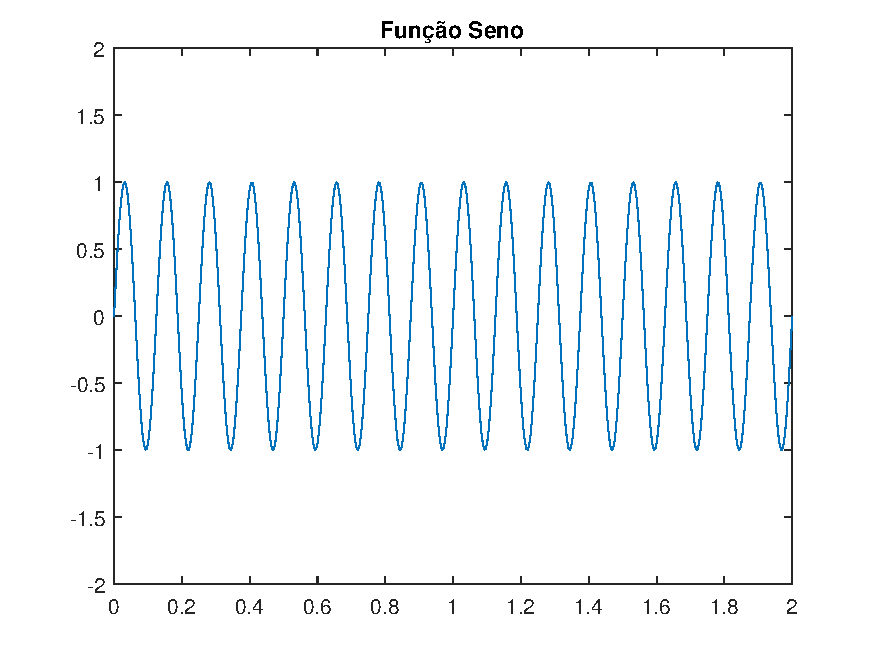
\includegraphics[width=\textwidth]{função seno.pdf}
        \caption{Função Seno.}
    \end{minipage}
    \hfill
    \begin{minipage}[b]{0.49\textwidth}
        \centering
        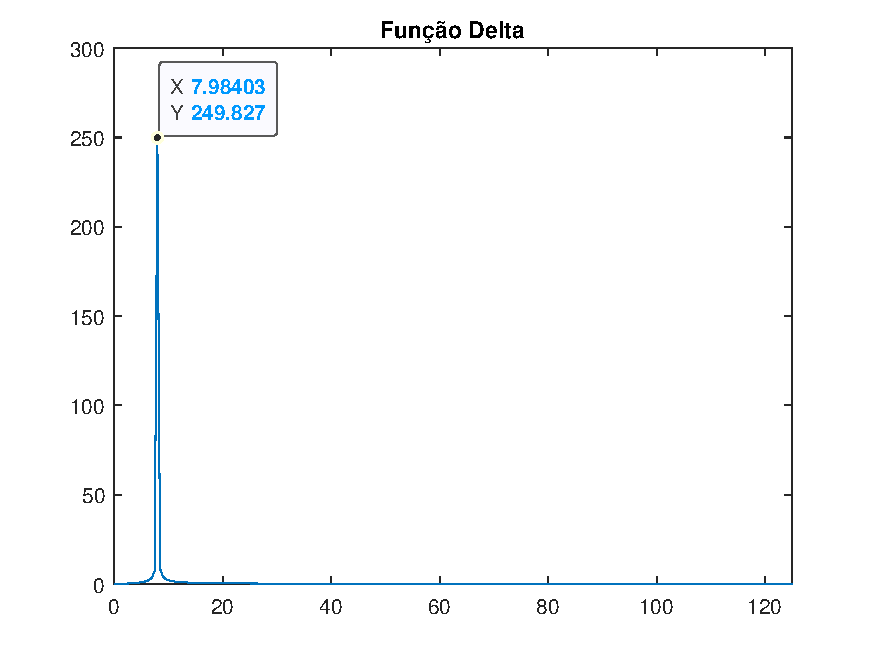
\includegraphics[width=\textwidth]{função delta.pdf}
        \caption{Função Delta.}
    \end{minipage}
\end{figure}

\subsection{Função Gaussiana}

A transformada de Fourier de uma função gaussiana é também uma função gaussiana mas com parâmetros diferentes.

\lstinputlisting[style=Matlab-editor, basicstyle=\small, caption={Slide 13.}, label={lst: gauss}, firstline=2]{./codigo/gauss.m}

Neste caso, a amplitude da transformada de Fourier é 5 e a média é 125. As figuras da página seguinte mostram a resposta do código apresentado.

\newpage

\begin{figure}[!ht]
    \centering
    \begin{minipage}[b]{0.49\textwidth}
        \centering
        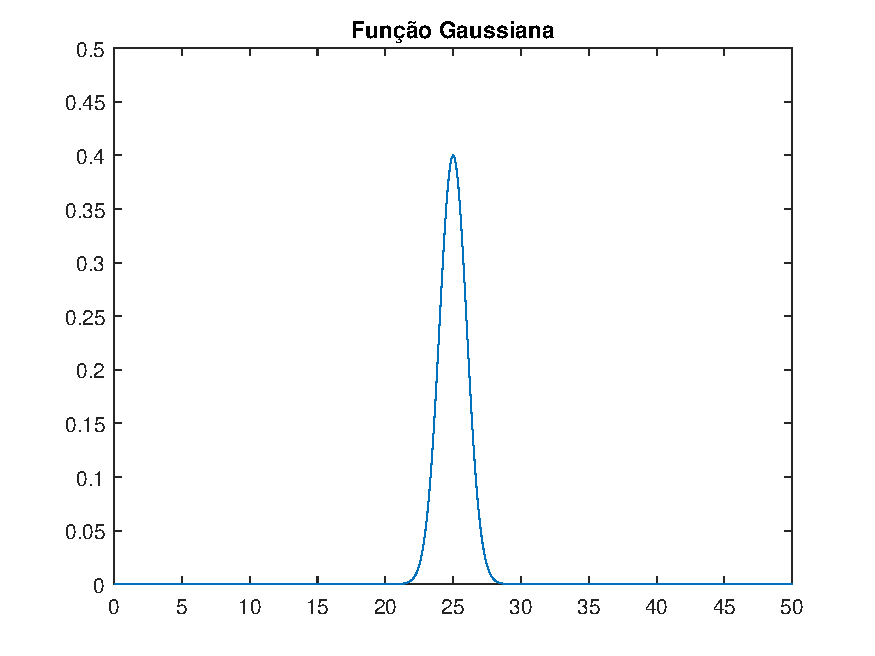
\includegraphics[width=\textwidth]{gauss.pdf}
        \caption{Função Gaussiana.}
    \end{minipage}
    \hfill
    \begin{minipage}[b]{0.49\textwidth}
        \centering
        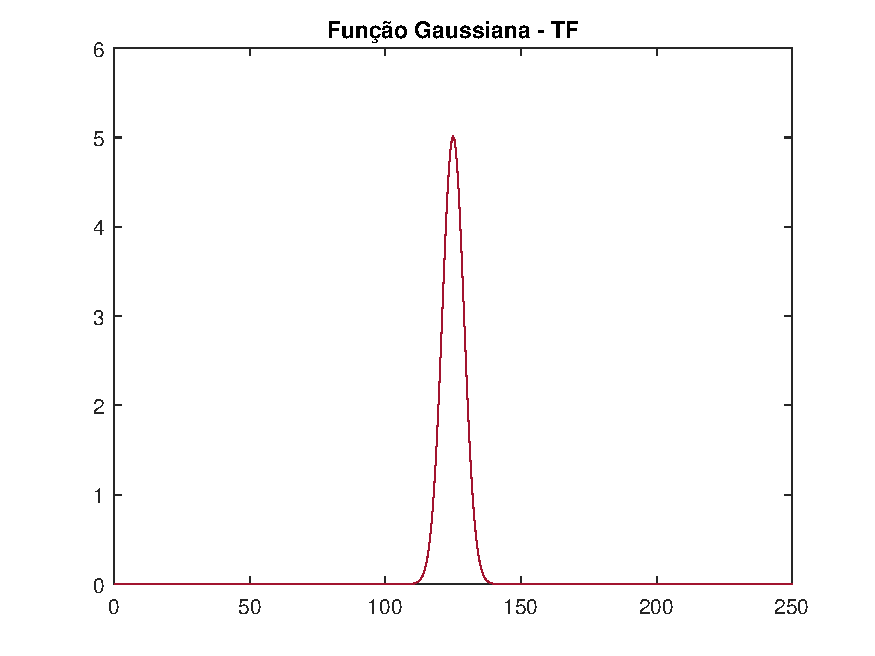
\includegraphics[width=\textwidth]{gaussTF.pdf}
        \caption{Função Gaussiana - TF.}
    \end{minipage}
\end{figure}

\subsection{Função Seno Cardinal \boldmath{$\rightarrow$} \emph{Square Wave}}

\lstinputlisting[style=Matlab-editor, basicstyle=\small, caption={Slides 14 e 15.}, label={lst: sinc_ped}, firstline=2]{./codigo/sinc_ped.m}

A transformada de Fourier da função seno cardinal (sinc) resulta numa \emph{square wave} (pedestal). 

De forma intuitiva, a função seno cardinal tem oscilações até ao infinito e quando a sua transformada de Fourier é calculada, envolve a soma de componentes sinusoidais infinitas, o que resulta numa onda quadrada. 

Essencialmente, a transformada de Fourier da função seno cardinal capta a propriedade fundamental desta função, nomeadamente o seu comportamento oscilatório, que no eixo das frequências, resulta numa \emph{square wave}.

\begin{figure}[!ht]
\centering
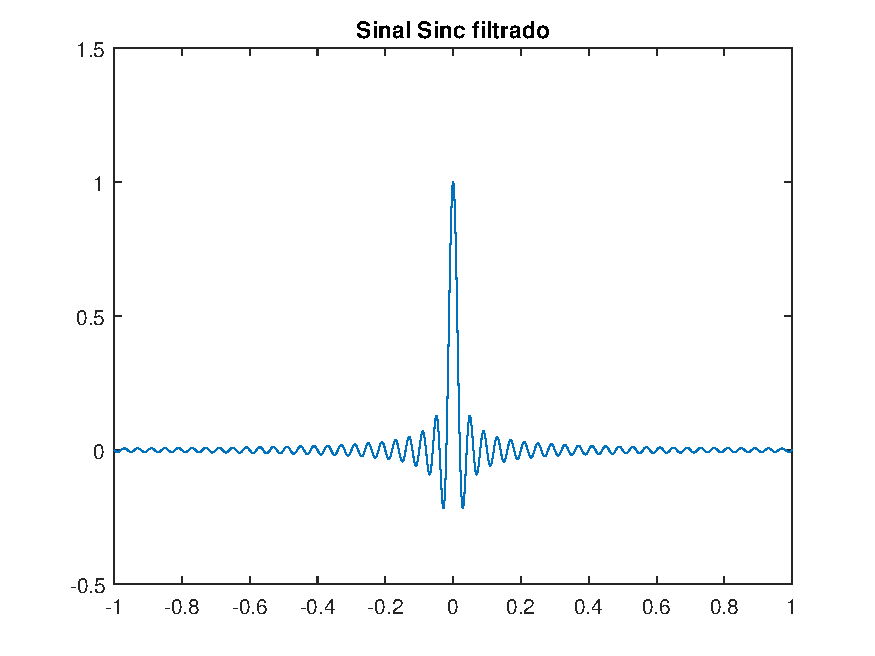
\includegraphics[width=0.75\textwidth]{sinc.pdf}
\caption{Função Sinc.}
\end{figure}

\begin{figure}[!ht]
    \centering
    \begin{minipage}[b]{0.49\textwidth}
        \centering
        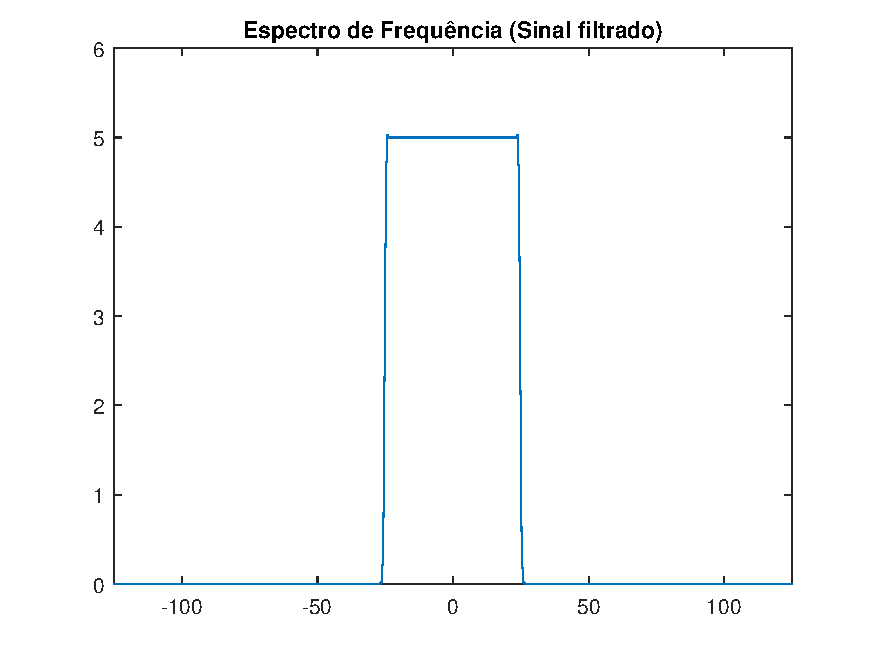
\includegraphics[width=\textwidth]{sinc2.pdf}
        \caption{Espectro de Frequências.}
    \end{minipage}
    \hfill
    \begin{minipage}[b]{0.49\textwidth}
        \centering
        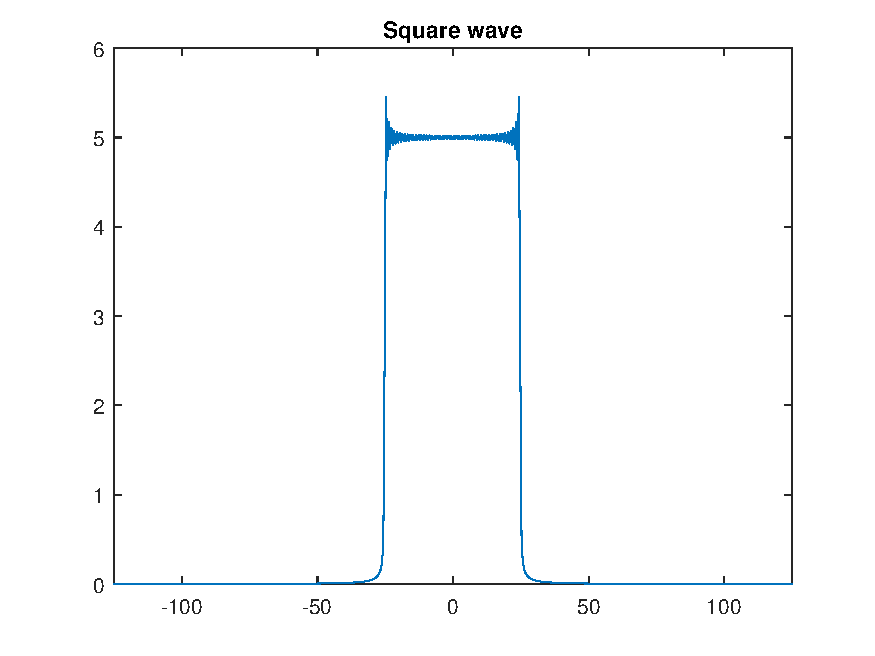
\includegraphics[width=\textwidth]{sinc3.pdf}
        \caption{Square Wave.}
    \end{minipage}
\end{figure}

\newpage

\subsection{Função Exponencial \boldmath{$\rightarrow$} Lorentziana}

\lstinputlisting[style=Matlab-editor, basicstyle=\small, caption={Slide 16.}, label={lst: exp_lorentz}, firstline=2]{./codigo/exp_lorentz.m}

\begin{figure}[!ht]
    \centering
    \begin{minipage}[b]{0.49\textwidth}
        \centering
        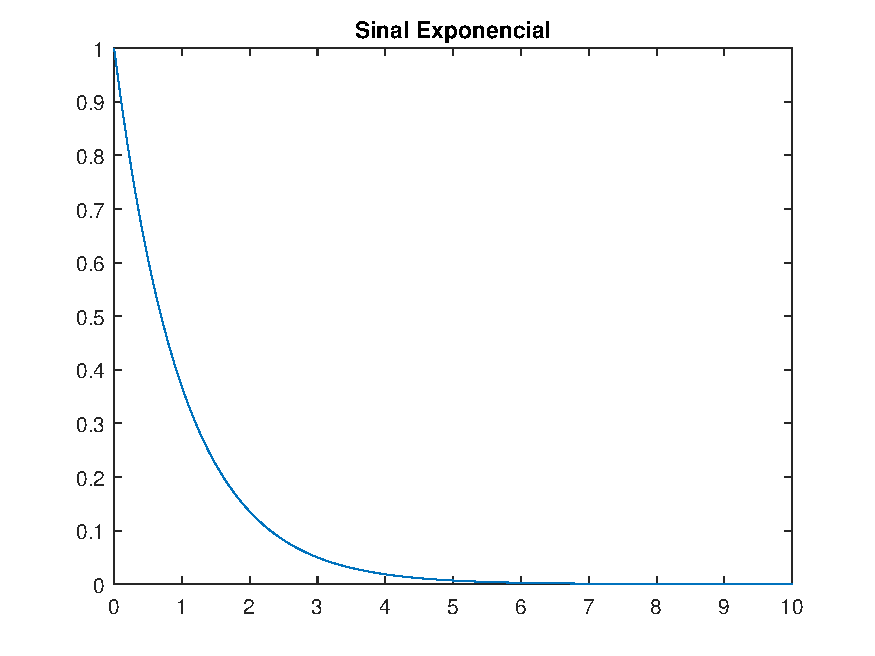
\includegraphics[width=\textwidth]{exp_lorentz1.pdf}
        \caption{Função Exponencial.}
    \end{minipage}
    \hfill
    \begin{minipage}[b]{0.49\textwidth}
        \centering
        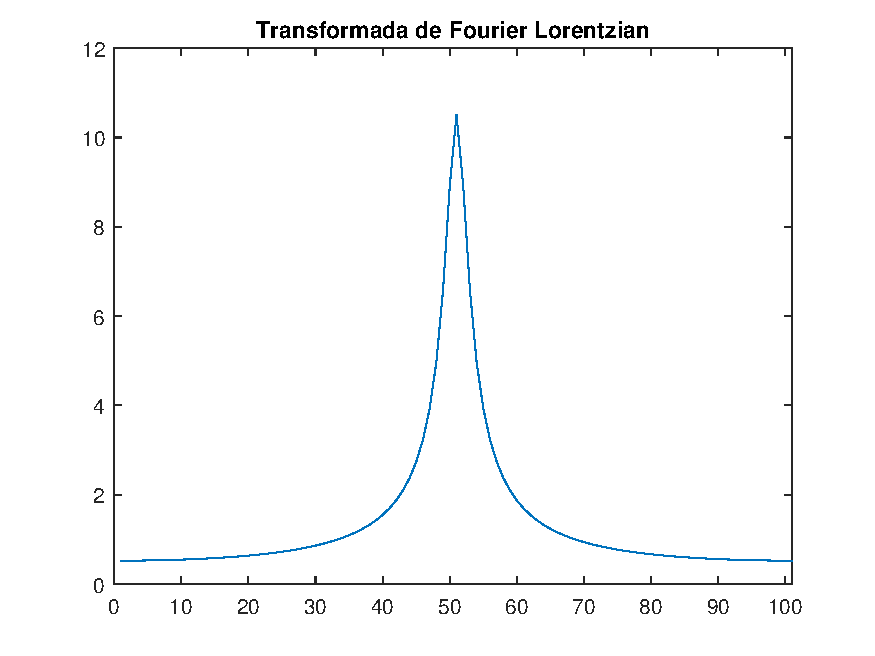
\includegraphics[width=\textwidth]{exp_lorentz2.pdf}
        \caption{Lorentziana.}
    \end{minipage}
\end{figure}

\section{FFT ou FID}